\documentclass[10pt]{article}
\usepackage{fullpage}
\usepackage{amsmath}
\usepackage[amsthm, thmmarks]{ntheorem}
\usepackage{amssymb}
\usepackage{graphicx}
\usepackage{enumerate}
\usepackage{verse}
\usepackage{tikz}
\usepackage{verbatim}
\usepackage{hyperref}
\usepackage{bbm}

\newtheorem{lemma}{Lemma}
\newtheorem{theorem}[lemma]{Theorem}
\newtheorem{definition}[lemma]{Definition}
\newtheorem{proposition}[lemma]{Proposition}
\newtheorem{corollary}[lemma]{Corollary}
\newtheorem{claim}[lemma]{Claim}
\newtheorem{example}[lemma]{Example}

\newcommand{\dee}{\mathrm{d}}
\newcommand{\Dee}{\mathrm{D}}
\newcommand{\In}{\mathrm{in}}
\newcommand{\Out}{\mathrm{out}}
\newcommand{\pdf}{\mathrm{pdf}}
\newcommand{\Cov}{\mathrm{Cov}}
\newcommand{\Var}{\mathrm{Var}}

\newcommand{\ve}[1]{\mathbf{#1}}
\newcommand{\ves}[1]{\boldsymbol{#1}}
\newcommand{\mrm}[1]{\mathrm{#1}}
\newcommand{\etal}{{et~al.}}
\newcommand{\sphere}{\mathbb{S}^2}
\newcommand{\modeint}{\mathcal{M}}
\newcommand{\azimint}{\mathcal{N}}
\newcommand{\ra}{\rightarrow}
\newcommand{\mcal}[1]{\mathcal{#1}}
\newcommand{\X}{\mathcal{X}}
\newcommand{\Y}{\mathcal{Y}}
\newcommand{\Z}{\mathcal{Z}}
\newcommand{\x}{\mathbf{x}}
\newcommand{\y}{\mathbf{y}}
\newcommand{\z}{\mathbf{z}}
\newcommand{\tr}{\mathrm{tr}}
\newcommand{\sgn}{\mathrm{sgn}}
\newcommand{\diag}{\mathrm{diag}}
\newcommand{\Real}{\mathbb{R}}
\newcommand{\sseq}{\subseteq}
\newcommand{\ov}[1]{\overline{#1}}
\newcommand{\data}{\mathrm{data}}

\DeclareMathOperator*{\argmin}{arg\,min}


\title{Neural Jacobian Fields}
\author{Pramook Khungurn}

\begin{document}
\maketitle


This note is written as I read the paper ``Neural Jacobian Fields: Learning Intrinsic Mappings of Arbitrary Meshes'' by Aigerman \etal~\cite{Aigerman:2022}.

\section{Preliminary}

\begin{itemize}
    \item This paper presents a framework to generate ``piecewise linear mappings'' of meshes with a neural network.
    
    \item In this note, we treat points in $\Real^d$ as \emph{row vectors}.
    \begin{itemize}
        \item So, if $\ve{x} \in \Real^3$, then
        \begin{align*}
            \ve{x} = \begin{bmatrix}
                x^1 & x^2 & x^3
            \end{bmatrix}.
        \end{align*}

        \item Notice that we use superscripts to denote components of a vector. This is because we will use subscripts for other things.

        \item This means that a linear transformation from $\Real^3$ to $\Real^2$ is encoded with a $3 \times 2$ matrix instead of $2 \times 3$. This matrix is multiplied to the right instead of to the left.
    \end{itemize}

    \item This makes it quite convenient to represent a batch of $N$ points and matrices.
    \begin{itemize}
        \item A batch of $N$ points in $\Real^3$ is represented by a matrix $\ve{P}$ of size $N \times 3$.
        \item A linear transformations from $\Real^3$ to $\Real^2$ is represented by a matrix $M$ fo size $3 \times 2$.
        \item If we wish to apply this linear transformation to all points in the batch, we just compute $\ve{P} M$.
    \end{itemize}    
\end{itemize}

\subsection{Meshes}

\begin{itemize}
    \item Let us formally define what a mesh is.
    \begin{itemize}
        \item We are given a triangular mesh $\mcal{S}$ in $\Real^3$ with vertices $\ve{V}$ and triangles $\ve{T}$.
        \item The $i$th triangle in $\ve{T}$ is denoted by $\ve{t}_i$.
        \item The {\bf tangent space} of $\ve{t}_i$ is the linear space orthogonal to its normal. It is denoted by $T_i$.
        \begin{itemize}
            \item Bascially, this is the plane in $\Real^3$ that the triangle lies in.
        \end{itemize}
        \item A {\bf frame} of triangle $\ve{t}_i$ is an oriented orthonomal basis fo its tangent space. It is denoted by $\mcal{B}_i$.
        \begin{itemize}
            \item We don't actually know in which direction the frame points to.
            \item I guess the natural direction is the direction of the normal vector.            
        \end{itemize}
    \end{itemize}

    \item Let's talk about how the tangent space is represented numerically.
    \begin{itemize}
        \item Let us say that the three vertices of $\ve{t}_i$ have indices $j$, $k$, and $l$.
        
        \item So, the triangle vertices are $\ve{v}_j$, $\ve{v}_k$, and $\ve{v}_l$.
        
        \item Let us also say that we designate $\ve{v}_j$ is the origin of tangent space $T_i$.
        
        \item So, we have that $T_i = \{ a(\ve{v}_k - \ve{v}_j) + b(\ve{v}_l - \ve{v}_j) : a, b \in \Real \}$.
        \begin{itemize}
            \item Here, we see that $T_i$ is a set of vectors because $\ve{v}_k - \ve{v}_j$ and $\ve{v}_l - \ve{v}_j$ are vectors.            
        \end{itemize}
        
        \item $\mcal{B}_i$ is an orthonomal basis of $T_i$. So, we may say that it is a $2 \times 3$ matrix:
        \begin{align*}
            \mcal{B}_i = \begin{bmatrix}
                \ves{\beta}_{i,1} \\ 
                \ves{\beta}_{i,2}
            \end{bmatrix}            
        \end{align*}
        where $\ves{\beta}_{i,1}, \ves{\beta}_{i,2} \in \Real^{3}$ such that $\| \ves{\beta}_{i,1} \| = \| \ves{\beta}_{i,2} \| = 1$ and $\ves{\beta}_{i,1} \cdot \ves{\beta}_{i,2} = 1$. Last but not least, $T_i = \{ a \ves{\beta}_{i,1} + b \ves{\beta}_{i,2} : a, b \in \Real \}.$
        
        \item Because $\mcal{B}_i$ is an orthonormal basis of $T_i$, we have that, for any vector $\ve{v} \in T_i$, we can find the coordinates of $\ve{v}$ with respect to $\mcal{B}_i$ as follows:
        \begin{align*}
            \mbox{$\ve{v}$'s coordinate} = \ve{v} \mcal{B}_i^T.
        \end{align*}

        \item Moreover, for any $\ve{x} \in \Real^3$, we have that
        \begin{align*}
            (\ve{x} - \ve{v}_j) \mcal{B}_i^T \mcal{B}_i
        \end{align*}
        is the projection of $\ve{x} - \ve{v}_j$ onto the plane of the triangle $\ve{t}_i$. As a result,
        \begin{align*}
            \ve{v}_j + (\ve{x} - \ve{v}_j) \mcal{B}_i^T \mcal{B}_i
        \end{align*}
        is the point on the plane of the triangle $\ve{t}_i$ that is the closest to $\ve{x}$.        
    \end{itemize}
\end{itemize}

\subsection{Linear Piecewise Mapping}

\begin{itemize}    
    \item A {\bf map} or a {\bf mapping}, in our context, is a function $\ves{\Phi}: \Real^{3} \ra \Real^{3}$.
    
    \item We can think of $\ves{\Phi}$ as being composed of three maps of signature $\Real^d \ra \Real$, one for each component of the output. We can denote the components by $\Phi^1$, $\Phi^2$, and $\Phi^3$. In this way, we have that
    \begin{align*}
        \ves{\Phi}(\ve{x}) = \begin{bmatrix} \Phi^1(\ve{x}) & \Phi^2(\ve{x}) & \Phi^3(\ve{x}) \end{bmatrix}
    \end{align*}
    
    \item A map $\ves{\Phi}$ is a {\bf piecewise linear mapping} with respect to a mesh $\mcal{S}$ if the restriction of $\ves{\Phi}$ to any triangle $\ve{t}_i$, denote $\ves{\Phi}|_{\ve{t}_i}$ is affine.
    \begin{itemize}
        \item This is the most common family of maps used when considering mappings of meshes.        
    \end{itemize}

    \item A piecewise linear mapping is uniquely defined by assigning a new position to one of the vertices.
    \begin{itemize}
        \item In other words, let $\ve{v}_j$ denote the position of the $j$th vertex. Suppose that we know $\ves{\Phi}_j$, the image of $\ve{v}_j$ under the mapping, for all $j$.
        
        \item Then, any point inside the triangle is sent to the interpolation of the $\ves{\Phi}_j$s with barycentric coordinates.            
        
        \item As a result, we may encode $\ves{\Phi}$ as a matrix of the same dimension as $\ve{V}$.
        
        \item In this case, $\ves{\Phi}$ is a matrix of size $|\ve{V}| \times 3$.
    \end{itemize}

    \item Another way to look at the piecewise linear mapping is to see it as a linear combination of basis functions.
    \begin{itemize}
        \item The basis function we use in this case is called the {\bf hat function}.
        
        \begin{itemize}
            \item  For each Vertex $j$, we define the hat function $\varphi_j$ to be a piecewise linear function on each triangle where $\varphi_j(\ve{v}_j) = 1$ and $\varphi_j(\ve{v}_k) = 0$ for all $k \leq j$. See Figure~\ref{fig:hat-function}.
        \end{itemize}
        
        \begin{figure}
        \begin{center}
        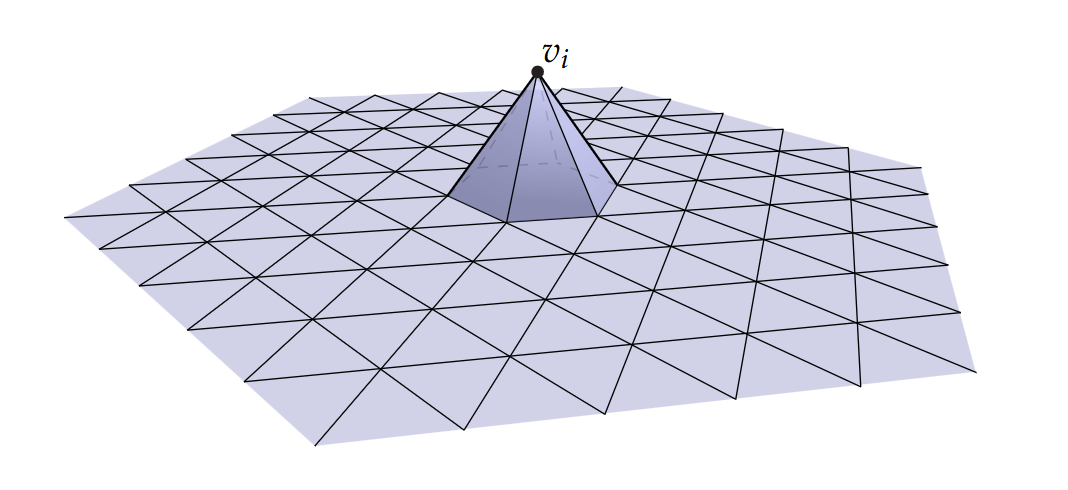
\includegraphics[width=5in]{images/hat-function.png}
        \end{center}
        \caption{The hat function.}
        \label{fig:hat-function}
        \end{figure}
        
        \item So, the piecewise linear mapping $\ves{\Phi}$ can be written as:
        \begin{align*}
            \ves{\Phi}(\ve{x}) = \sum_{j=1}^{|\ve{V}|} \ves{\Phi}_j \varphi_j(\ve{x}).
        \end{align*}

        \item Remember that $\ves{\Phi}$ has three component functions. Each function can also be written as a linear combination of the hat functions as well.
        \begin{align*}
            \Phi^1(\ve{x}) &= \sum_{j=1}^{|\ve{V}|} \Phi_j^1 \varphi_j(\ve{x}), &
            \Phi^2(\ve{x}) &= \sum_{j=1}^{|\ve{V}|} \Phi_j^2 \varphi_j(\ve{x}), &
            \Phi^3(\ve{x}) &= \sum_{j=1}^{|\ve{V}|} \Phi_j^3 \varphi_j(\ve{x})
        \end{align*}
    \end{itemize}
\end{itemize}

\subsection{Gradients}

\begin{itemize}
    \item Let us define a {\bf scalar field} to be a function of signature $\Real^3 \ra \Real$.
    \item A scalar field is {\bf piecewise linear} if, when restricted to each triangle in a mesh, it is an affine function.
    \item We also know that any piecewise linear scalar field can be written as a linear combination of hat functions.
    \item We have that, for a piecewise linear mapping $\ves{\Phi}$, its component functions $\Phi^1$, $\Phi^2$, and $\Phi^3$ are piecewise linear scalar fields.
    \item Consider a piecewise linear scalar field $f$. It is meaningful to talk about its gradient
    \begin{align*}
        \nabla f(\ve{x}) = \begin{bmatrix}
            \nabla_1 f(\ve{x}) \\
            \nabla_2 f(\ve{x}) \\
            \nabla_3 f(\ve{x})
        \end{bmatrix}.        
    \end{align*}
    Here, because a vector is a row vector, so a gradient should be a column vector.

    \item Let $f|_{\ve{t}_i}$ denote $f$ restricted to Triangle $\ve{t}_i$. From definition, $f|_{\ve{t}_i}$ is an affine function. As a result, $\nabla f|_{\ve{t}_i}$ is a constant vector. In particular,
    \begin{align*}
        \nabla f|_{\ve{t}_i} = (f_k - f_j) \frac{\ve{v}_j - \ve{v}_l}{A(\ve{t}_i)} + (f_l - f_j) \frac{\ve{v}_k - \ve{v}_j}{A(\ve{t}_i)}
    \end{align*}
    where $j,k,l$ are indices of the vertices of $\ve{t}_i$, and $A(\ve{t}_i)$ is the area of $\ve{t}_i$.

    \item Because $f$ can be encoded as a $|\ve{V}| \times 1$ matrix, we can encode $\nabla f$ with a $3|\ve{T}| \times 1$ matrix.
    
    \item $\nabla$ is a linear operator, so it can be encoded with a $3|\ve{T}| \times |\ve{V}|$ matrix.
    
    \item The \texttt{grad} function from the libigl library~\cite{libigl:2025} computes this matrix.
\end{itemize}

\subsection{Poisson Problem on a Mesh}

\begin{itemize}
    \item Recall that a {\bf Poisson problem} is the following mathmatical problem.
    \begin{itemize}
        \item We are given a domain $\Omega \subseteq \Real^3$.
        \item We are also given a vector field $\ve{g}: \Omega \ra \Real^3$.
        \item We are to find a scalar field $f: \Omega \ra \Real$ that minimizes the following energy:
        \begin{align*}
            \int_{\Omega} \| \nabla f(\ve{x}) - \ve{g}(\ve{x}) \|^2\, \dee \ve{x}.
        \end{align*}
    \end{itemize}
    In other words, we are asked to find a scalar field whose gradient fits the given vector field the best.

    \item It can be shown that the optimal function $f^*$ satisfies the following {\bf Poisson equation}:
    \begin{align*}
        \Delta f^*(\ve{x}) = \nabla \cdot \ve{g}(\ve{x})
    \end{align*}
    for all $\ve{x} \in \Omega$. Here, $\Delta$ is the Laplace operator:
    \begin{align*}
        \Delta f(\ve{x}) = \nabla \cdot \nabla f(\ve{x}) 
        = \sum_{i=1}^3 \frac{\partial^2 f(\ve{x})}{(\partial x^i)^2}
        = \sum_{i=1}^3 \nabla_i \nabla_i f(\ve{x})
        = \sum_{i=1}^3 \nabla_{i,i} f(\ve{x}),
    \end{align*}
    and $\nabla \cdot$ is the divergence operator
    \begin{align*}
        \nabla \cdot \ve{g}(\ve{x}) = \sum_{i=1}^3 \frac{\partial \ve{g}^i(\ve{x})}{\partial x^i} = \sum_{i=1}^3 \nabla_i g^i(\ve{x})
    \end{align*}

    \item We note that $f^*$ is unique up to a constant shift. This because
    \begin{align*}
        \nabla (f + c) = \nabla f
    \end{align*}
    for all constant $c \in \Real$.

    \item On a mesh, the Poisson problem takes on a different guise.
    \begin{itemize}
        \item We are given a mesh $\mathcal{S}$.
        \item We are given a vector field $\ve{g}$, that is supposed to encode the gradient of a piecewise linear scalar field.
        \begin{itemize}
            \item This is encoded as a $3|\ve{T}| \times 1$ matrix.            
        \end{itemize}
        \item We are supposed to find a piecewise linear scalar field $f$ that minimizes the following energy
        \begin{align*}
            \int_{\mathcal{S}} \| \nabla f(\ve{x}) - \ve{g}(\ve{x}) \|^2 \, \dee\ve{x}
            &= \sum_{i=1}^{|\ve{T}|} A(\ve{t}_i) \| (\nabla f)_i - \ve{g}_i \|^2.
        \end{align*}
        where $(\nabla f)_i$ and $\ve{g}_i$ denote the values of the corresponding vector fields at triangle $\ve{t}_i$.
    \end{itemize}

    \item We can show that, the optimal piecewise linear scalar field $f^*$ must satisfy the equation
    \begin{align*}
        \nabla f^* = \nabla \cdot \ve{g}.
    \end{align*}
    Here, $\nabla \cdot$ is a matrix that represents the divergence operator. It is a $|\ve{V}| \times 3|\ve{T}|$ matrix that is equal to
    \begin{align*}
        \nabla \cdot = \nabla^T \mcal{A}
    \end{align*}
    where $\mcal{A}$ is a $3|\ve{T}| \times 3|\ve{T}|$ diagonal matrix that contains the area $A(\ve{t}_i)$ of the triangle $\ve{t}_i$ in the rows associated with the triangle $\ve{t}_i$. $\Delta$ is the $|\ve{V}| \times |\ve{V}|$ matrix that represents the Laplacian operator. It is equal to
    \begin{align*}
        \Delta = \nabla^T \mcal{A} \nabla.
    \end{align*}
    It can be shown that this is equal to the ``cotangent Laplacian'' that is widely used in discrete differential geometry \cite{Crane:DdgCourse:2025}.

    \item So, we can find $f^*$ by computing
    \begin{align*}
        f^* = \Delta^{-1} \nabla^T \mcal{A}\ve{g}.
    \end{align*}
    
    \item However, the above equation doesn't quite work because $\Delta$ is a not a full-rank matrix because, if you add the columns up, you will get a zero vector. So, any linear solver would complain.
    
    \item The way to solve this is to do the following.
    \begin{enumerate}
        \item Trim $\Delta$ down to a $(|\ve{V}|-1) \times (|\ve{V}|-1)$ matrix and $\Delta^T \mcal{A}$ by lobbing off its 1st row and 1st column.
        \item Trim $\nabla^T \mcal{A}$ to a $(|\ve{V}|-1) \times 3|\ve{T}|$ by lobbing off its 1st row.
        \item Compute $f^* = \Delta^{-1} \nabla^T \mcal{A}\ve{g}$ with a standard linear solver.
        \item The output is a $|\ve{V}-1| \times 1$ matrix. To get a full response, just add an extra row of $0$ at the beginning.
    \end{enumerate}
    Note that, for the last step, $0$ is the only one value that would work. (Think about the $(|\ve{V}|-1) \times (|\ve{V}|-1)$ version of $\Delta$ being a submatrix of the full $\Delta$.)

    \item In other words, given a vector field that is supposed to be the gradient of some piecewise linear scalar field over a mesh, we can find a piecewise linear scalar field whose gradient is the closest to tha vector field by solving a linear equation.
\end{itemize}

\subsection{Jacobians}
    
\begin{itemize}        
    \item We learned earlier that a piecewise linear mapping $\ves{\Phi}$ is made up of three piecewise linear scalar fields $\Phi^1$, $\Phi^2$, and $\Phi^3$.
    
    \item Let us take a look at the derivative of $\ves{\Phi}$, denoted by $\nabla \ves{\Phi}$ and commonly called the {\bf Jacobian} of $\ves{\Phi}$.
    \begin{align*}
        \nabla \ves{\Phi}(\ve{x}) = \begin{bmatrix}
            \nabla_1 \Phi^1(\ve{x}) & \nabla_1 \Phi^2(\ve{x}) & \nabla_1 \Phi^3(\ve{x}) \\
            \nabla_2 \Phi^1(\ve{x}) & \nabla_2 \Phi^2(\ve{x}) & \nabla_2 \Phi^3(\ve{x}) \\
            \nabla_3 \Phi^1(\ve{x}) & \nabla_3 \Phi^2(\ve{x}) & \nabla_3 \Phi^3(\ve{x})
        \end{bmatrix}
        &= \begin{bmatrix}
            \nabla \Phi^1(\ve{x}) & \nabla \Phi^2(\ve{x}) & \nabla \Phi^3(\ve{x})
        \end{bmatrix}.
    \end{align*}
    So, the Jacobian of $\ves{\Phi}$ is the stack of gradient vectors of its component functions, which are scalar fields over the mesh.

    \item Again, if we restrict $\ves{\Phi}$ to a triangle $\ve{t}_i$, we have that $\nabla \Phi^1|_{\ve{t}_i}(\ve{x})$, $\nabla \Phi^2|_{\ve{t}_i}(\ve{x})$, $\nabla \Phi^3|_{\ve{t}_i}(\ve{x})$ are constant vectors, which we will denote by $(\nabla\Phi^1)_i$, $(\nabla\Phi^2)_i$, and $(\nabla\Phi^3)_i$. So,
    \begin{align*}
        \nabla \ves{\Phi}|_{\ve{t}_i}(\ve{x})
        &= \begin{bmatrix}
            (\nabla \Phi^1)_i & (\nabla \Phi^2)_i & (\nabla \Phi^3)_i
        \end{bmatrix}.
    \end{align*}
    As a result, $\nabla \ves{\Phi}|_{\ve{t}_i}(\ve{x})$ is a constant, which we will denote by $(\nabla \ves{\Phi})_i$. 

    \item Thus, we can represent the Jacobian of piecewise linear mapping $\ves{\Phi}$ by a $|\ve{T}| \times 3 \times 3$ tensor or, to agree with the convention in the previous section, a $3|\ve{T}| \times 3$ matrix.
    
    \item As a result, given field of $3 \times 3$ matrices $\ve{M}$ over a mesh, which is represent by assigning a $3 \times 3$ matrix to each triangle, we can find a piecewise linar mapping $\Phi^*$ such that its Jacobian matrices are closes to $\ve{M}$ by computing
    \begin{align*}
        \ves{\Phi}^* = \Delta^{-1} \nabla^T \mcal{A} \ve{M}.
    \end{align*}
    This is equivalent to solving the problems for each component functions $(\Phi^*)^1$, $(\Phi^*)^2$, $(\Phi^*)^3$ independently.

    \item Let's see what we have so far.
    \begin{itemize}
        \item If we have a piecewise linear mapping $\ves{\Phi}$, we can difinite compute its Jacobian matrices $\ve{M} = \nabla \ves{\Phi}$, which is an assignment of each triangle to a $3 \times 3$ matrix.
        \item On the other hand, if we have $\mcal{M}$, which is a stack of $3 \times 3$ matrices where there is one for each triangle, then we can find a piecewise linear mapping $\Phi^*$ such that $\nabla \Phi^*$ is the closest to $M$.
    \end{itemize}
    Moreover, if we do $\ves{\Phi} \ra \ve{M} \ra \ves{\Phi}^*$, we have that $\ves{\Phi}$ and $\ves{\Phi}^*$ only differs by a translation.

    \item As a result, it follows that we can encode a piecewise linear transformation by its Jacobian matrices.
    \begin{itemize}
        \item Of course, we have to figure out the missing translation somehow, but we will worry about that later.
    \end{itemize}
\end{itemize}

\subsection{Restricting Jacobians to Tangent Spaces}

\begin{itemize}
    \item Recall that Jacobians are linear transformation such that
    \begin{align*}
        \ves{\Phi}(\ve{x} + \ve{h}) \approx \ves{\Phi}(\ve{x}) + \ve{h} \nabla \ves{\Phi}(\ve{x})
    \end{align*}
    when $\ve{h}$ is small enough.

    \item When we restrict $\ves\Phi$ to the triangle $\ve{t}_i$, we have that $\ves\Phi|_{\ve{t}_i}$ is an affine function, and so the approximation above becomes exact.
    \begin{align*}
        \ves{\Phi}|_{\ve{t}_i}(\ve{x} + \ve{h}) 
        = \ves{\Phi}|_{\ve{t}_i}(\ve{x}) + \ve{h} \nabla \ves{\Phi}|_{\ve{t}_i}(\ve{x}) 
        = \ves{\Phi}|_{\ve{t}_i}(\ve{x}) + \ve{h} (\nabla \ves{\Phi})_i.
    \end{align*}

    \item We typically understand the small vector $\ve{h}$ as a vector in the tangent space of $\ve{x}$. In other words,
    \begin{align*}
        \ve{h} = \ve{b} \mcal{B}_i
    \end{align*}
    where $\ve{b} \in \Real^2$ and $\mcal{B}_i$ is the matrix of basis vectors of the tangent space $T_i$ of triangle $\ve{t}_i$.

    \item Thus,
    \begin{align*}
        \ves{\Phi}|_{\ve{t}_i}(\ve{x} + \ve{b}\mcal{B}_i)         
        = \ves{\Phi}|_{\ve{t}_i}(\ve{x}) + \ve{b} \mcal{B}_i (\nabla \ves{\Phi})_i.
    \end{align*}

    \item We can view $\mcal{B}_i(\nabla \ves{\Phi})_i$ as a restriction of the Jacobian $(\nabla \ves{\Phi})_i$ so that it operates on vectors in the tangent space of the triangle $\ve{t}_i$. This matrix is a $2 \times 3$ matrix.
    
    \item In particular, let us say that we have the stack $\mcal{B}$ of the basis matrices of the tangent spaces, and this is a $|\ve{T}| \times 2 \times 3$ tensor. Suppose that $\nabla \ves{\Phi}$ is represented by a $|\ve{T}| \times 3 \times 3$ tensor. Then, the restrictions of the Jacobian matrices to the tangent spaces are given by
    \begin{align*}
        \texttt{bmm}(\mcal{B}, \ves{\Phi})
    \end{align*}
    where $\texttt{bmm}$ denotes the batch matrix multiplication function, implemented in PyTorch and other deep learning frameworks.
\end{itemize}

\section{Method}

\subsection{The Big Picture}

\begin{itemize}
    \item The goal of the paper is to create a neural network that consumes a mesh and produces a piecewise linear mapping of the mesh.    
    
    \item We know what the output looks like. It is $\ves{\Phi}$, which assigns each vertex of the mesh to a point in $\Real^3$. However, we will make our life easier by saying that the position of the new mesh can be arbitrary in space; i.e., we remove the translation of the mesh.
    
    \item With the relaxed requirement, we can encode a piecewise linear mapping with the field of $3\times3$ Jacobian matrices over the triangles.
    
    \item The paper chooses to predict the Jacobian field instead of the new positions of each vertex. Once the Jacobian field has been predicted, one can get a position assignment by solving Poisson's equation.
    
    \item The main goal of the paper is to make sure that {\bf how the prediction gets done should be agnostic to the triangulation of the mesh.}
    \begin{itemize}
        \item This means that the triangles in the mesh should not be processed as a whole.
    \end{itemize}

    \item As a result, the paper proposes a network that processes each triangle independently.
    \begin{itemize}
        \item It takes in information regarding the centroid of the triangle.
        \begin{itemize}
            \item Position.
            \item Normal vector.
            \item Wave-Kernel signature (WKS) \cite{Aubry:WKS:2011} of size 50, computed by averaging the WKSs of the three triangle vertices.
        \end{itemize}

        \item In order for the network to have access to global information about the mesh, it also takes in a {\bf global code} $\ve{z}$, which is the same for all triangles.
        \begin{itemize}
            \item We will talk about the global codes later.
        \end{itemize}

        \item The network then should predict a $3 \times 3$ matrix, which serves as the Jacobian matrix of the predicted piecewise linear mapping.
    \end{itemize}

    \item The global code can contains information about many things.
    \begin{itemize}        
        \item The shape of the input mesh.
        \begin{itemize}
            \item The paper uses the encoding by PointNet \cite{Qi:PointNet:2017}.
            \begin{itemize}
                \item We sample $1024$ points on the mesh.
                \item We create a tensor of point information. Each entry corresponds to a point and has the following fields: (1) the point's 3D position, (2) the point's normal vector, and (3) the point's Wave-Kernel signature \cite{Aubry:WKS:2011} of size 50.
                \item We feed the above tensor to PointNet to get an encoding.            
            \end{itemize}                    
        \end{itemize}

        \item The shape of the output mesh. This can be encoded in the same way as the shape of the input mesh.
        
        \item It can also incorporate conditioning information $\ve{y}$ such as the desired pose of the output mesh, the joint angles of the skeleton, desired position to which mesh should bend to, and so on.        
    \end{itemize}

    \item So, in the end, we need to train the following networks
    \begin{itemize}
        \item A {\bf mesh encoder} $E$ that maps the shape of the input mesh and other conditioning information (shape of the output mesh, desired pose, etc.) to a {\bf global code} $\ve{z}$.
        \item A {\bf mapper} $M$ that takes in the global code $\ve{z}$ and centroid features $\ve{c}_i$ and output the Jacobian of that triangle $J_i$.
    \end{itemize}

    \item Note that the above two networks do not have to know how many triangles there are in the mesh or how the triangles are connected.
    \begin{itemize}
        \item The mesh encoder only process samples on the surface of the mesh.
        \item The mapper processes each triangles independently. It only knows the centroid of the triangle, not the vertices that the triangles are connected to.
    \end{itemize}
\end{itemize}

\subsection{The Specifics}

\begin{itemize}
    \item The training data is a collection of tuples $\{ \mcal{S}, \ves{\Psi}, \ve{y} \}$ where
    \begin{itemize}
        \item $\mcal{S}$ is a mesh, which has the following information.
        \begin{itemize}
            \item The vertex positions $\ve{V} = (\ve{v}_1, \ve{v}_2, \dotsc)^T$.
            \item The triangles $\ve{T} = (\ve{t}_1, \ve{t}_2, \dotsc)^T$.
            \item Information about surface samples $\ve{S} = (\ve{s}_1, \ve{s}_2, \dotsc)^T$ as required by PointNet.
            \item Information about centroids $\ve{C} = (\ve{c}_1, \ve{c}_2, \dotsc)^T$.
            \item The matrix of its gradient operator $\nabla$.
            \item Its mass matrix $\mcal{A}$.
            \item The matrix of its divergence operator $D = \nabla^T \mcal{A}$.
            \item The matrix of its Laplacian operator $L = \nabla^T \mcal{A} \nabla$.
            \begin{itemize}
                \item This matrix prefactored to allow for fast linear solving.
            \end{itemize}
        \end{itemize}
        \item $\ves{\Psi}$ is the groundtruth mapping, which is basically an assignment of each vertex in $\mcal{S}$ to a new position.
        \item $\ve{y}$ is a conditioning information.
    \end{itemize}

    \item Given a mesh $\mcal{S}$, the prediction is conducted as follows.
    \begin{itemize}
        \item We first use the encoder to produce the latent code: $\ve{z} = E(\ve{S}, \ve{y})$.
        \item For each triangle $\ve{t}_i$ in the mesh, we compute a $3\time3$ Jacobian matrix $J_i = M(\ve{c}_i, \ve{z})$.
        \begin{itemize}
            \item Let us denote the stack of $J_i$s by $\ve{J}$.
        \end{itemize}
        \item We then compute a linear piecewise mapping by solving Poisson's equation:
        \begin{align*}
                L \ves{\Phi} = D \ve{J}.
        \end{align*}
        \item We return $\ves{\Phi}$ as the output.
    \end{itemize}

    \item Training uses the following loss.
    \begin{align*}
        \mcal{L} = \lambda_{\mrm{vertex}} \mcal{L}_{\mrm{vertex}} + \mcal{L}_{\mrm{jacobian}}
    \end{align*}
    \begin{itemize}
        \item $\mcal{L}_{\mrm{vertex}}$ is L2 loss between the predicted vertex positions and the ground-truth ones.
        \begin{itemize}
            \item The paper uses the formula
            \begin{align*}
                \mcal{L}_{\mrm{vertex}} = \sum_{j=1}^{|\ve{V}|} m(\ve{v}_j) \| \ves{\Phi}_j - \ves{\Psi}_j \|^2.
            \end{align*}
            where $m(\ve{v}_j)$ is the ``lumped mass'' around Vertex $\ve{v}_j$.
            \item However, in the code, there is no lumped mass term. The formula is just:
            \begin{align*}
                \mcal{L}_{\mrm{vertex}} = \sum_{j=1}^{|\ve{V}|} \| \ves{\Phi}_j - \ves{\Psi}_j \|^2
            \end{align*}
            \item Since the predicted mapping in unique up to translation, it is translated so that the center of mass are the same.
        \end{itemize}

        \item $\mcal{L}_{\mrm{vertex}}$ is the L2 loss between the Jacobian matrices, restricted to the tangent space of each traingle.
        \begin{itemize}
            \item The paper uses the formula
            \begin{align*}
                \mcal{L}_{\mrm{vertex}} = \sum_{i=1}^{|\ve{T}|} A(\ve{t}_i) \| \mcal{B}_i J_i - \mcal{B}_i (\nabla \Psi)_i \|^2.
            \end{align*}
            \item However, again, the code just drops the scaling factor.
            \begin{align*}
                \mcal{L}_{\mrm{vertex}} = \sum_{i=1}^{|\ve{T}|} \| \mcal{B}_i J_i - \mcal{B}_i (\nabla \Psi)_i \|^2.
            \end{align*}
        \end{itemize}

        \item The weight $\lambda$ is set to $10$ in the paper.
    \end{itemize}

    \item The mapping network $M$.
    \begin{itemize}
        \item This is a 5-layer fully connected MLP with ReLU activation and group norm after each leayer.
        \item Hidden layers are of size 128.
        \item The first layer depends on the size of $\ve{z}$.
        \item The last layer outputs 9 numbers.
        \item We add the identity matrix to output of the last layer so that the MLP still producees a valid matrix when it outputs the zero matrix (which it is likely to do right after initialization).        
    \end{itemize}

    \item The global code $\ve{z}$.
    \begin{itemize}
        \item It may contain raw conditioning information such as the pose of the output mesh.
        \item To encode shape of a mesh, the paper uses a PointNet \cite{Qi:PointNet:2017}.
        \begin{itemize}
            \item It receives 1024 points sampled uniformly on the mesh, along with their normals and WKS of size 50.
            \item The PointNet is modified to use group normalization.
            \item It is trained together with the mapping network.
        \end{itemize}
    \end{itemize}

    \item Training.
    \begin{itemize}
        \item The optimizer is Adam.
        \item Learning rate is first $10^{-3}$ until loss plateaus. Then, it is reduced to $10^{-4}$ and trained until the loss plateuas again.        
    \end{itemize}

    \item Factoring the Laplacian $L$.
    \begin{itemize}
        \item The paper says it uses LDL decomposition implemented by SciPy's SuperLU decomposition.
        \item However, the code uses \texttt{CholeskySolverD} from the \texttt{cholespy} library.
    \end{itemize}

\end{itemize}


\bibliographystyle{arxivalpha}
\bibliography{neural-jacobian-fields}  
\end{document}